\documentclass{ieeeaccess}
%DIF LATEXDIFF DIFFERENCE FILE
%DIF DEL /tmp/Main_old_6d4eee4f.tex   Thu Apr  2 23:55:31 2026
%DIF ADD Main.tex                     Thu Apr  2 23:45:47 2026
\usepackage{cite}
\usepackage{amsmath,amssymb,amsfonts}
\usepackage{algorithmic}
\usepackage{graphicx}
\usepackage{textcomp}

\usepackage{bm}
\makeatletter
\AtBeginDocument{\DeclareMathVersion{bold}
\SetSymbolFont{operators}{bold}{T1}{times}{b}{n}
\SetSymbolFont{NewLetters}{bold}{T1}{times}{b}{it}
\SetMathAlphabet{\mathrm}{bold}{T1}{times}{b}{n}
\SetMathAlphabet{\mathit}{bold}{T1}{times}{b}{it}
\SetMathAlphabet{\mathbf}{bold}{T1}{times}{b}{n}
\SetMathAlphabet{\mathtt}{bold}{OT1}{pcr}{b}{n}
\SetSymbolFont{symbols}{bold}{OMS}{cmsy}{b}{n}
\renewcommand\boldmath{\@nomath\boldmath\mathversion{bold}}}
\makeatother

\def\BibTeX{{\rm B\kern-.05em{\sc i\kern-.025em b}\kern-.08em
    T\kern-.1667em\lower.7ex\hbox{E}\kern-.125emX}}

\graphicspath{{img/}{../out/experiment1/}{../out/experiment2/}{../out/experiment4/}}
%DIF PREAMBLE EXTENSION ADDED BY LATEXDIFF
%DIF UNDERLINE PREAMBLE %DIF PREAMBLE
\RequirePackage[normalem]{ulem} %DIF PREAMBLE
\RequirePackage{color}\definecolor{RED}{rgb}{1,0,0}\definecolor{BLUE}{rgb}{0,0,1} %DIF PREAMBLE
\providecommand{\DIFadd}[1]{{\protect\color{blue}\uwave{#1}}} %DIF PREAMBLE
\providecommand{\DIFdel}[1]{{\protect\color{red}\sout{#1}}} %DIF PREAMBLE
%DIF SAFE PREAMBLE %DIF PREAMBLE
\providecommand{\DIFaddbegin}{} %DIF PREAMBLE
\providecommand{\DIFaddend}{} %DIF PREAMBLE
\providecommand{\DIFdelbegin}{} %DIF PREAMBLE
\providecommand{\DIFdelend}{} %DIF PREAMBLE
\providecommand{\DIFmodbegin}{} %DIF PREAMBLE
\providecommand{\DIFmodend}{} %DIF PREAMBLE
%DIF FLOATSAFE PREAMBLE %DIF PREAMBLE
\providecommand{\DIFaddFL}[1]{\DIFadd{#1}} %DIF PREAMBLE
\providecommand{\DIFdelFL}[1]{\DIFdel{#1}} %DIF PREAMBLE
\providecommand{\DIFaddbeginFL}{} %DIF PREAMBLE
\providecommand{\DIFaddendFL}{} %DIF PREAMBLE
\providecommand{\DIFdelbeginFL}{} %DIF PREAMBLE
\providecommand{\DIFdelendFL}{} %DIF PREAMBLE
\newcommand{\DIFscaledelfig}{0.5}
%DIF HIGHLIGHTGRAPHICS PREAMBLE %DIF PREAMBLE
\RequirePackage{settobox} %DIF PREAMBLE
\RequirePackage{letltxmacro} %DIF PREAMBLE
\newsavebox{\DIFdelgraphicsbox} %DIF PREAMBLE
\newlength{\DIFdelgraphicswidth} %DIF PREAMBLE
\newlength{\DIFdelgraphicsheight} %DIF PREAMBLE
% store original definition of \includegraphics %DIF PREAMBLE
\LetLtxMacro{\DIFOincludegraphics}{\includegraphics} %DIF PREAMBLE
\newcommand{\DIFaddincludegraphics}[2][]{{\color{blue}\fbox{\DIFOincludegraphics[#1]{#2}}}} %DIF PREAMBLE
\newcommand{\DIFdelincludegraphics}[2][]{% %DIF PREAMBLE
\sbox{\DIFdelgraphicsbox}{\DIFOincludegraphics[#1]{#2}}% %DIF PREAMBLE
\settoboxwidth{\DIFdelgraphicswidth}{\DIFdelgraphicsbox} %DIF PREAMBLE
\settoboxtotalheight{\DIFdelgraphicsheight}{\DIFdelgraphicsbox} %DIF PREAMBLE
\scalebox{\DIFscaledelfig}{% %DIF PREAMBLE
\parbox[b]{\DIFdelgraphicswidth}{\usebox{\DIFdelgraphicsbox}\\[-\baselineskip] \rule{\DIFdelgraphicswidth}{0em}}\llap{\resizebox{\DIFdelgraphicswidth}{\DIFdelgraphicsheight}{% %DIF PREAMBLE
\setlength{\unitlength}{\DIFdelgraphicswidth}% %DIF PREAMBLE
\begin{picture}(1,1)% %DIF PREAMBLE
\thicklines\linethickness{2pt} %DIF PREAMBLE
{\color[rgb]{1,0,0}\put(0,0){\framebox(1,1){}}}% %DIF PREAMBLE
{\color[rgb]{1,0,0}\put(0,0){\line( 1,1){1}}}% %DIF PREAMBLE
{\color[rgb]{1,0,0}\put(0,1){\line(1,-1){1}}}% %DIF PREAMBLE
\end{picture}% %DIF PREAMBLE
}\hspace*{3pt}}} %DIF PREAMBLE
} %DIF PREAMBLE
\LetLtxMacro{\DIFOaddbegin}{\DIFaddbegin} %DIF PREAMBLE
\LetLtxMacro{\DIFOaddend}{\DIFaddend} %DIF PREAMBLE
\LetLtxMacro{\DIFOdelbegin}{\DIFdelbegin} %DIF PREAMBLE
\LetLtxMacro{\DIFOdelend}{\DIFdelend} %DIF PREAMBLE
\DeclareRobustCommand{\DIFaddbegin}{\DIFOaddbegin \let\includegraphics\DIFaddincludegraphics} %DIF PREAMBLE
\DeclareRobustCommand{\DIFaddend}{\DIFOaddend \let\includegraphics\DIFOincludegraphics} %DIF PREAMBLE
\DeclareRobustCommand{\DIFdelbegin}{\DIFOdelbegin \let\includegraphics\DIFdelincludegraphics} %DIF PREAMBLE
\DeclareRobustCommand{\DIFdelend}{\DIFOaddend \let\includegraphics\DIFOincludegraphics} %DIF PREAMBLE
\LetLtxMacro{\DIFOaddbeginFL}{\DIFaddbeginFL} %DIF PREAMBLE
\LetLtxMacro{\DIFOaddendFL}{\DIFaddendFL} %DIF PREAMBLE
\LetLtxMacro{\DIFOdelbeginFL}{\DIFdelbeginFL} %DIF PREAMBLE
\LetLtxMacro{\DIFOdelendFL}{\DIFdelendFL} %DIF PREAMBLE
\DeclareRobustCommand{\DIFaddbeginFL}{\DIFOaddbeginFL \let\includegraphics\DIFaddincludegraphics} %DIF PREAMBLE
\DeclareRobustCommand{\DIFaddendFL}{\DIFOaddendFL \let\includegraphics\DIFOincludegraphics} %DIF PREAMBLE
\DeclareRobustCommand{\DIFdelbeginFL}{\DIFOdelbeginFL \let\includegraphics\DIFdelincludegraphics} %DIF PREAMBLE
\DeclareRobustCommand{\DIFdelendFL}{\DIFOaddendFL \let\includegraphics\DIFOincludegraphics} %DIF PREAMBLE
%DIF AMSMATHULEM PREAMBLE %DIF PREAMBLE
\makeatletter %DIF PREAMBLE
\let\sout@orig\sout %DIF PREAMBLE
\renewcommand{\sout}[1]{\ifmmode\text{\sout@orig{\ensuremath{#1}}}\else\sout@orig{#1}\fi} %DIF PREAMBLE
\makeatother %DIF PREAMBLE
%DIF COLORLISTINGS PREAMBLE %DIF PREAMBLE
\RequirePackage{listings} %DIF PREAMBLE
\RequirePackage{color} %DIF PREAMBLE
\lstdefinelanguage{DIFcode}{ %DIF PREAMBLE
%DIF DIFCODE_UNDERLINE %DIF PREAMBLE
  moredelim=[il][\color{red}\sout]{\%DIF\ <\ }, %DIF PREAMBLE
  moredelim=[il][\color{blue}\uwave]{\%DIF\ >\ } %DIF PREAMBLE
} %DIF PREAMBLE
\lstdefinestyle{DIFverbatimstyle}{ %DIF PREAMBLE
	language=DIFcode, %DIF PREAMBLE
	basicstyle=\ttfamily, %DIF PREAMBLE
	columns=fullflexible, %DIF PREAMBLE
	keepspaces=true %DIF PREAMBLE
} %DIF PREAMBLE
\lstnewenvironment{DIFverbatim}{\lstset{style=DIFverbatimstyle}}{} %DIF PREAMBLE
\lstnewenvironment{DIFverbatim*}{\lstset{style=DIFverbatimstyle,showspaces=true}}{} %DIF PREAMBLE
\lstset{extendedchars=\true,inputencoding=utf8}

%DIF END PREAMBLE EXTENSION ADDED BY LATEXDIFF

\begin{document}
\history{Date of publication xxxx 00, 0000, date of current version xxxx 00, 0000.}
\doi{10.1109/ACCESS.2024.0429000}

\title{A Real-Time Haptic Simulation Prototype for Liver Lesion Localization Training: System Design, Technical Feasibility Validation, and Formative Expert Evaluation}
\author{\uppercase{Siyu Wang}\authorrefmark{1},
\uppercase{Yunxiu Xu}\authorrefmark{1},
and \uppercase{Shoichi Hasegawa}\authorrefmark{1}}
\address[1]{Department of Information and Communication Engineering, Institute of Science Tokyo, Yokohama, Japan (e-mail: siw131@haselab.net, yunxiu@haselab.net, hasevr@haselab.net)}
\corresp{Corresponding author: Siyu Wang (e-mail: siw131@haselab.net).}

\begin{abstract}
Haptic feedback has potential value in medical training, but the feasibility of integrating physics computation into a real-time haptic loop remains insufficiently explored. To evaluate the system connectivity of a physics engine in an interactive palpation task, this study develops a task-oriented haptic training prototype. Using liver lesion localization as the application scenario, we adopt a group-based corotational finite element method as the physical model, combine it with bimanual tracking and a fingertip-worn interface, and establish a closed loop between large-deformation computation and force response. Hidden lesions are simulated through local modulus enhancement, and the extracted contact-normal reaction force is mapped to haptic output. All runtime tests were conducted on consumer-grade hardware, and a formative expert evaluation was performed to identify engineering boundaries. The results show that the prototype supports system-level operation driven by physics computation and demonstrate the feasibility of this haptic integration architecture and device deployment. Based on these findings, the discussion highlights the challenges that remain before the current physical model can be translated into a clinical-grade training system, including simplified anatomical constraints and the absence of nonlinear material properties, thereby providing design implications and engineering references for future medical palpation systems.
\end{abstract}

\begin{keywords}
Liver palpation, real-time simulation, corotational finite element method, haptic interaction, medical training.
\end{keywords}

\titlepgskip=-21pt
\maketitle

\section{Introduction}
Haptic feedback and soft-tissue simulation have long been regarded as important components of medical training systems, but their effectiveness does not depend only on whether haptics is present. It is closely related to task type, evaluation method, and feedback design. Existing reviews show that the value of haptic feedback is often more evident in complex tasks, while training outcomes are still influenced by device degrees of freedom, feedback realism, and experimental design \cite{overtoom2019haptic,rangarajan2020systematic,escobar2016review}. For liver lesion localization, operators must compare local stiffness differences under limited visual information. This makes the task a natural testbed for asking whether physics computation can be translated into perceivable haptic cues. Prior work has already shown that liver palpation diagnosis can itself serve as a standalone simulation target, and that liver-related interactive systems are not limited to resection or cutting tasks \cite{westwood2012haptic,hongyu2021interactive}.

From the computational perspective, soft tissues such as the liver exhibit pronounced large deformation and near-incompressible behavior during pressing and traction. Real-time simulation therefore faces a dual constraint of accuracy and efficiency. Continuum finite element methods (FEM) offer strong physical interpretability and are well suited to representing local stiffness changes and material-parameter differences, but traditional global solvers are expensive. To address this issue, prior research has explored corotational FEM, cutting FEM, and grouped solving strategies to preserve physical credibility under real-time constraints \cite{bui2019corotational,wang2025group}. At the same time, Projective Dynamics, position-based dynamics (PBD), and extended position-based dynamics (XPBD) offer advantages in interactive speed, numerical stability, and implementation convenience \cite{bouaziz2023projective,liu2016towards,bender2014survey,muller2007position,macklin2016xpbd}. However, when the goal is to represent lesion stiffness rather than merely visually plausible motion, material interpretability and mechanical consistency remain central.

From the interaction perspective, high-degree-of-freedom (DOF) force-feedback devices can provide richer kinesthetic and contact information, but they usually come with engineering costs such as structural complexity, high price, and restricted workspace \cite{agboh2016six}. Review studies likewise indicate that medical training systems do not necessarily benefit from blindly pursuing the highest number of degrees of freedom or the highest possible fidelity. What matters more is whether the critical perceptual cues are emphasized for a specific task \cite{overtoom2019haptic,rangarajan2020systematic}. Recent work also stresses task-oriented force-profile design rather than reconstructing every haptic dimension by default \cite{bjelland2025haptic}. This provides theoretical support for the one-degree-of-freedom (1-DOF) interface used here: if lesion search depends primarily on local differences in normal resistance, then low-complexity hardware may still play a meaningful role in preclinical validation.

\DIFaddbegin \DIFadd{From the educational perspective, training for practical medical skills such as palpation faces challenges of real-case shortages and ethical risks. Practical teaching requires a reproducible practice environment. As Chernikova }\emph{\DIFadd{et al.}} \DIFadd{\mbox{%DIFAUXCMD
\cite{chernikova2020simulation} }\hskip0pt%DIFAUXCMD
pointed out, simulation-based learning shows positive utility in higher education, and a large amount of practice is a necessary requirement for developing professional skills. This study constructs a real-time physical computation loop based on consumer-grade hardware, not merely pursuing cost control, but aiming to break the physical space and equipment quantity limitations imposed by traditional medical simulators, satisfying the actual demand in medical education to popularize high-frequency haptic simulation training in daily classrooms.
}

\DIFadd{In addition to practice frequency, the educational field has equally strict demands for feedback quality. When medical novices practice on traditional plastic models, they often receive only static tactile sensations, lacking dynamic guidance. Wisniewski }\emph{\DIFadd{et al.}} \DIFadd{\mbox{%DIFAUXCMD
\cite{wisniewski2020power} }\hskip0pt%DIFAUXCMD
noted that the impact of feedback on learning achievement is directly influenced by the information content it conveys. This system achieves low-latency computation, and by establishing a closed loop between FEM large-deformation computation and force response, the system can output dynamic, real-time, and physics-rich haptic feedback to the learner's fingertips based on modulus changes of internal liver lesions. Such immediate haptic feedback based on tissue mechanics directly responds to the theoretical demand for high-information feedback in educational psychology, assisting learners in establishing mental representations of hand perception and internal lesions.
}

\DIFaddend Overall, existing studies provide foundations in real-time soft-tissue modeling, liver-related training tasks, and medical haptic-system design, but relatively few works integrate a physically meaningful continuum model, \DIFdelbegin \DIFdel{consumer-grade }\DIFdelend interactive large-deformation updating, and a \DIFdelbegin \DIFdel{lightweight }\DIFdelend haptic loop into a single task-oriented system framework \DIFaddbegin \DIFadd{that directly addresses these educational demands}\DIFaddend .

Based on this motivation, this paper proposes and implements a task-oriented haptic training prototype to evaluate the system connectivity and engineering feasibility of integrating continuum physics computation into a lightweight haptic loop\DIFaddbegin \DIFadd{, aiming to meet the educational demands for high-frequency practice and high-information physical feedback}\DIFaddend . The prototype uses liver lesion localization as a concrete test scenario, adopts a group-based corotational finite element method (GB-cFEM) as the core physical engine, combines it with Stereo IR-170 bimanual tracking and a haptic interface, simulates hidden lesions via local modulus enhancement, and maps contact-normal reaction force to haptic output. The evaluation in this paper is a formative expert evaluation whose goal is to identify system feasibility and engineering boundaries. The main contributions are as follows:
\begin{enumerate}
\item A task-oriented GB-cFEM physical-haptic closed-loop system prototype is proposed and implemented. \DIFdelbegin \DIFdel{Contact-normal force is extracted from a continuum physics engine and translated into force output, demonstrating the system connectivity of this computational architecture for palpation interaction and }\DIFdelend \DIFaddbegin \DIFadd{By }\DIFaddend enabling real-time deployment on compact consumer-grade hardware\DIFaddbegin \DIFadd{, this architecture responds to the educational demand for hardware accessibility, establishing the foundation for popularizing high-frequency haptic simulation training in routine classrooms}\DIFaddend .
\item A haptic mapping and exploration mechanism for lesion localization is designed. By \DIFdelbegin \DIFdel{combining simulated differences in stiffness between lesions and surrounding tissue with }\DIFdelend \DIFaddbegin \DIFadd{extracting contact-normal forces from a continuum physics engine and translating them into dynamic force output via }\DIFaddend a fingertip-worn \DIFdelbegin \DIFdel{haptic }\DIFdelend interface, the system \DIFdelbegin \DIFdel{supports real-time extraction and feedback of hidden-lesion mechanical features and demonstrates the application potential of }\DIFdelend \DIFaddbegin \DIFadd{provides high-information physical feedback based on }\DIFaddend regional hardness differences\DIFdelbegin \DIFdel{as palpation cues}\DIFdelend \DIFaddbegin \DIFadd{, assisting learners in interpreting internal lesion mechanics}\DIFaddend .
\item A formative evaluation involving a surgical expert is conducted. Through walkthrough-based assessment, the study evaluates the prototype's ability to transform FEM-based stiffness into recognizable mechanical cues and identifies the engineering boundaries and practical constraints that remain before translation to a clinical-grade trainer.
\end{enumerate}

\section{Related Work}
Interactive simulation systems for surgical training and palpation-skill acquisition typically require engineering tradeoffs among visual rendering rate, haptic update frequency, and physical-modeling complexity. Reviews in this area note that virtual-reality and haptic-feedback systems for medical training are limited not only by tissue-mechanics modeling and real-time rendering, but also by task definition, evaluation methodology, and the maturity of educational evidence \cite{overtoom2019haptic,rangarajan2020systematic,escobar2016review}. For the liver palpation training task studied here, the most relevant research threads concern real-time soft-tissue modeling, liver-related training tasks, and low-dimensional haptic rendering.

\subsection{Real-Time Soft-Tissue Modeling for Surgical Simulation}
In soft-tissue modeling for surgical simulation, continuum FEM is a standard class of methods because it naturally represents material parameters, boundary conditions, and volumetric mesh structure, although it becomes computationally expensive under large deformation, near incompressibility, contact, and cutting. Corotational FEM separates large rotation from strain computation and achieves a favorable balance between efficiency and deformation quality, and has been used in real-time surgical settings such as needle insertion \cite{bui2019corotational}. Most directly relevant to this work is GB-cFEM, which combines grouped solving, domain decomposition, and offline precomputation to support large tetrahedral models, anisotropic materials, and near-incompressible cases on multicore CPUs \cite{wang2025group}. This makes it especially suitable as the core of the liver large-deformation simulation used here.

Beyond traditional FEM, Projective Dynamics and its extensions for hyperelastic materials also provide a balance between stability and real-time performance \cite{bouaziz2023projective,liu2016towards}, while soft-tissue models based on constraint energies further improve physical consistency in tool-tissue interaction \cite{hou2019new}. By comparison, PBD and XPBD are often used as engineering baselines in real-time systems because of their implementation simplicity and numerical robustness \cite{bender2014survey,muller2007position,macklin2016xpbd}. However, when anisotropy, near-incompressible volume preservation, and organ-level physical interpretability are required, FEM generally remains the more appropriate primary model.

\subsection{Liver-Related Simulation Systems and Training Tasks}
In interactive simulation for the liver and other abdominal organs, previous studies span both organ deformation and cutting workflows and palpation-based lesion exploration and training. Prior work has reported a liver-parenchymal transection system with haptic feedback \cite{hongyu2021interactive}, while another study presented a haptic simulation system for liver diagnosis through palpation \cite{westwood2012haptic}. These studies indicate that liver-related training is not limited to cutting. Palpation, localization, and stiffness comparison also have independent training value. Accordingly, the present work does not attempt to reproduce a full hepatectomy workflow, but instead focuses on the more clearly defined and more readily evaluable subtask of hidden-lesion palpation and localization.

\subsection{Haptic Device Degrees of Freedom and Low-Dimensional Haptic Rendering}
In medical haptic rendering, device degrees of freedom, force-mapping strategy, and system complexity are tightly coupled. Existing reviews describe both multi-DOF force-feedback interfaces and lightweight low-cost solutions \cite{overtoom2019haptic,rangarajan2020systematic,escobar2016review}. For example, Agboh \emph{et al.} proposed a six-DOF laparoscopic training interface, demonstrating the feasibility of high-DOF haptic reconstruction \cite{agboh2016six}. At the same time, growing evidence suggests that perceptual cues should be selected according to the task goal rather than assuming that full-dimensional, high-fidelity reconstruction is always necessary. Beyond traditional desktop devices, recent work has also proposed a lightweight fingernail-worn haptic device that provides force and vibration cues while minimizing obstruction of the natural fingerpad contact area, offering a new hardware path for low-burden bare-hand interaction \cite{xu2025lightweight}.

Along this line of reducing haptic dimensionality or emphasizing specific cues, reality-based force profiles have been used to simplify kinesthetic rendering in surgical simulation \cite{bjelland2025haptic}. These studies suggest that low-DOF haptic output is not merely a simplified substitute, but can also be understood as a task-oriented design choice for highlighting perceptual cues such as normal resistance and variation in stiffness from place to place.

\subsection{Position of This Work}
In summary, existing studies have established important foundations in real-time soft-tissue modeling, liver-related training tasks, and medical haptic rendering. However, there is still room to explore \DIFdelbegin \DIFdel{system-level integration of }\DIFdelend \DIFaddbegin \DIFadd{how to effectively integrate }\DIFaddend a physics engine \DIFdelbegin \DIFdel{and a lightweight }\DIFdelend \DIFaddbegin \DIFadd{with a }\DIFaddend haptic loop under consumer-grade hardware \DIFdelbegin \DIFdel{, together with system-level diagnosis}\DIFdelend \DIFaddbegin \DIFadd{to fulfill the educational demands of high-frequency practice and high-information physical feedback}\DIFaddend . Based on this gap, this paper develops a task-oriented haptic training prototype using liver lesion localization as the test scenario\DIFdelbegin \DIFdel{and focuses on validating }\DIFdelend \DIFaddbegin \DIFadd{. The focus is to validate }\DIFaddend the system integration and usability of a physics-computation-driven interaction architecture \DIFaddbegin \DIFadd{that aims to provide accessible and physics-rich mechanical cues for medical training}\DIFaddend . The evaluation in this paper is a formative expert evaluation whose goal is to identify system feasibility and engineering boundaries rather than to demonstrate training efficacy.

\section{System Design and Implementation}
\subsection{Overall System Architecture}
The system consists of four layers: a real-time physics simulation layer, an interaction input layer, a haptic rendering layer, and a task configuration layer. The real-time physics simulation layer uses GB-cFEM to solve the liver tetrahedral mesh in real time. The interaction input layer uses a Stereo IR-170 (Ultraleap, UK) to capture bimanual hand pose, with the five fingertips of the right hand corresponding to five virtual proxy spheres. The haptic rendering layer sends the contact-normal reaction force to a 1-DOF device through a serial protocol. The task configuration layer organizes blind lesion-localization experiments by switching among internal hard-region positions.

\subsection{Real-Time Simulation Core}
GB-cFEM is adopted as the real-time simulation core. The liver tetrahedral mesh is first divided into multiple local groups, each of which is solved independently in a corotational coordinate system for local deformation. During the offline stage, system matrices are calculated. At runtime, the main operations are rotation extraction, right-hand-side construction, and iterative computation. Continuity across groups is maintained through coupling constraints. Compared with a full global implicit FEM, this design avoids reassembling and refactorizing a large linear system every frame. Compared with XPBD, it preserves clearer material-parameter meaning and is therefore better suited to representing stiffness differences between normal tissue and lesion regions.

\subsection{Bimanual Input and Virtual Palpation Interaction}
The system uses the Stereo IR-170 for bimanual tracking. Fingertips are mapped to capsule-shaped proxy bodies used for local pressing, lesion localization, and surgical-field exposure. The right hand is primarily responsible for palpation and comparison, while the left hand is used mainly to push and retract tissue so as to create a local exposure window for the right hand to enter. To reduce tracking noise and the numerical shock caused by instantaneous penetration, the proxy bodies are not set equal to the raw sensor positions. Instead, they are connected to the device-side positions through damped virtual couplings.

\subsection{1-DOF Haptic Rendering Strategy}
The contact-normal reaction force is used as the main input to the 1-DOF device. The fingertip-worn haptic device used here follows the lightweight fingernail haptic design proposed by the authors previously. In this design, a motor drives a fine wire to apply normal force on the fingerpad side, while the lightweight actuation mechanism is integrated on the fingernail side to minimize occlusion of the fingerpad and reduce interference with natural touching behavior \cite{xu2025lightweight}. Because optical hand tracking has difficulty accurately distinguishing little-finger motion and can generate erroneous feedback, the experimental haptic device was implemented on the four fingers of the right hand except the little finger. On this basis, the device is further integrated into the real-time GB-cFEM simulation loop to convey differences in stiffness during the lesion-search task. The system extracts the contact-force vector $\mathbf{F}_{contact}$ and the surface normal $\mathbf{n}$ from the simulation core and computes the normal reaction-force magnitude delivered to the haptic hardware as
\begin{equation}
F_n = \left| \mathbf{F}_{contact} \cdot \mathbf{n} \right|.
\end{equation}
In the deployed system, the actual update rate of the haptic control loop is 1000 Hz, and the physics engine transmits force commands to the haptic hardware through a serial link at 2{,}000{,}000 bps. Under this mechanism, users perform lesion localization by perceiving differences in normal resistance while pressing different regions. The hardware connections and wearable device used in the experiment are shown in Fig.~\ref{fig:hardware}.

\begin{figure}[htbp]
\centerline{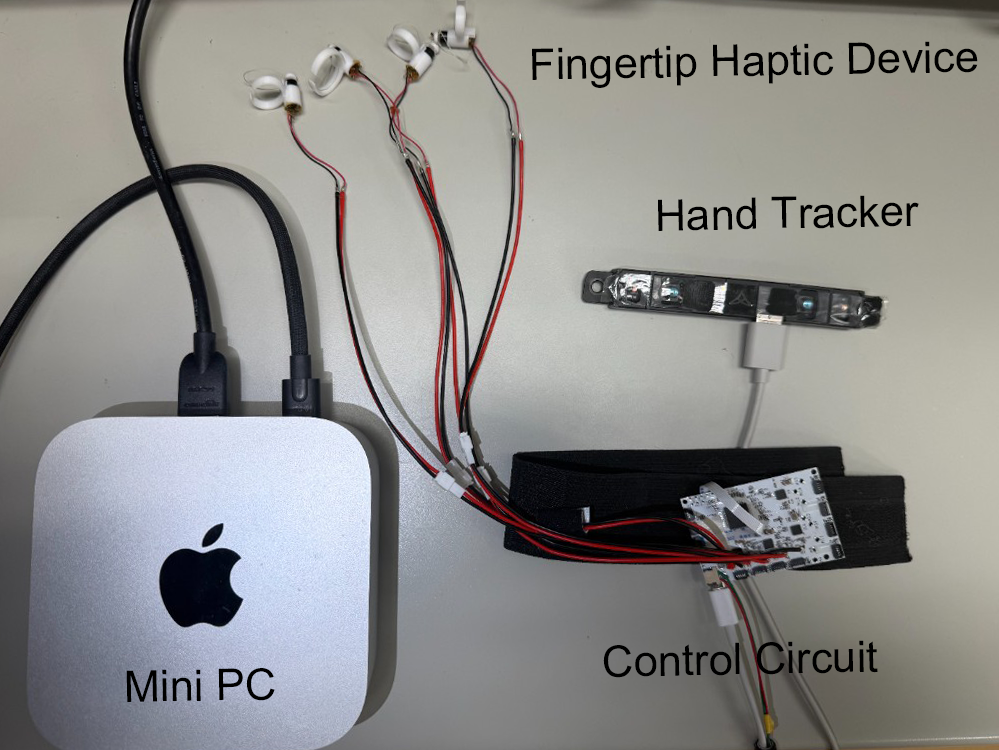
\includegraphics[width=0.9\linewidth]{hardware_and_wearable_device.png}}
\caption{Hardware setup used in the experiment. The lower-right part shows the wrist-mounted fixture and driving circuit, while the upper part shows the fingertip haptic actuator. Together with Stereo IR-170 tracking, the system provides hand tracking and normal-force cues.}
\label{fig:hardware}
\end{figure}

\subsection{Liver Model and Lesion Configuration}
Under the default configuration used in the physician experience session, the main system parameters are listed in Table~\ref{tab:model}. These parameters are intended to support a stable and perceptible interactive demonstration and are grounded in the deformation and volume behavior demonstrated by the underlying technical validation. In particular, the ``tetrahedral volume constraint correction'' in Table~\ref{tab:model} is not an inherent analytic property of the main GB-cFEM solver. It is an additional stabilization step enabled in the current system. This helps prevent local collapse, abnormal shrinkage, and subsequent contact jitter. The evaluation of the system in this paper therefore comes both from algorithm-level validation data and from the task performance and subjective feedback of a clinical expert during actual interaction.

\begin{table}[htbp]
\caption{Liver Model and Lesion Parameters Under the Default Physician-Experience Configuration}
\label{tab:model}
\centering
\footnotesize
\renewcommand{\arraystretch}{1.15}
\begin{tabular}{|p{0.22\linewidth}|p{0.20\linewidth}|p{0.46\linewidth}|}
\hline
Parameter & Value & Description \\
\hline
Geometry source & NIH 3D (3DPX-021007) & Open liver anatomy model \\
\hline
Meshing parameter & TetGen \texttt{-pq20a0.00}\allowbreak\texttt{0083} & Controls tetrahedral mesh quality and density \\
\hline
Base Young's modulus & 7000 Pa & Baseline stiffness of normal liver tissue \\
\hline
Tumor-region Young's modulus & 30000 Pa & Local stiffness enhancement in hard regions \\
\hline
Poisson ratio & 0.49 & Near-incompressible setting \\
\hline
Number of groups & 288 & Local grouped-solving configuration \\
\hline
Time step & 0.008 s & Real-time simulation step \\
\hline
Tetrahedral volume constraint correction & Enabled (2 iterations, correction = 0.15) & Pulls tetrahedra back toward their rest volume in each step to suppress local collapse, inversion, and abnormal shrinkage under deep pressing \\
\hline
\end{tabular}
\end{table}

To support blind localization experiments, the system presets three switchable local hard-region positions inside the liver. The hard regions are not indicated by visible geometric shape, but are hidden inside the tissue through embedded Young's-modulus enhancement. This forces participants to rely only on local deformation and haptic differences to infer lesion location. In addition to lesion configuration, fixed points are defined in three anatomical regions of the liver model to suppress nonphysical global drift and approximate basic attachment relations: the Porta Hepatis, the Groove for the Inferior Vena Cava (IVC groove), and the Bare Area, as shown in Fig.~\ref{fig:fixed}. This multi-point, surface-based anchoring strategy approximates the stable connection between the liver and major vascular and diaphragmatic attachment regions while preserving local deformability.

Beyond these anatomical anchors, a static liver-shaped abdominal support boundary is also introduced to approximate the external constraints imposed by surrounding abdominal tissue. Specifically, the system extracts the contact surface from the outer triangular mesh of the liver in the rest pose and offsets it outward along the surface normal of each facet by a distance proportional to the bounding-box diagonal, thereby constructing an envelope shell that follows the liver geometry while being slightly expanded. This shell is not designed as a fully closed abdominal box. A local opening is retained along a selected direction and serves as an exposure window created after incision and retraction, allowing fingers to enter from the exposed side for palpation.

At runtime, contact between surface vertices and this static shell is computed through local adjacent-triangle search and closest-point projection. Each vertex is required to stay on the interior side of the shell. When the projection indicates that a vertex has moved to the exterior of the shell by more than a small threshold along the local outward normal, the system applies a push-back correction along that normal, combined with tangential damping and velocity update to suppress oscillation. Accordingly, the ``abdominal collision'' in this paper should be understood more precisely as a liver-shaped support envelope generated from the rest-pose geometry rather than a high-fidelity anatomical reconstruction of the abdominal wall, diaphragm, and surrounding organs. This is also one of the main limitations of the current model. Although it provides more plausible spatial support than a simple planar wall, it does not yet model the anterior falciform ligament or authentic abdominal contact relations individually. The runtime interface and the division of left-hand exposure and right-hand palpation are shown in Fig.~\ref{fig:system}.

\begin{figure}[htbp]
\centerline{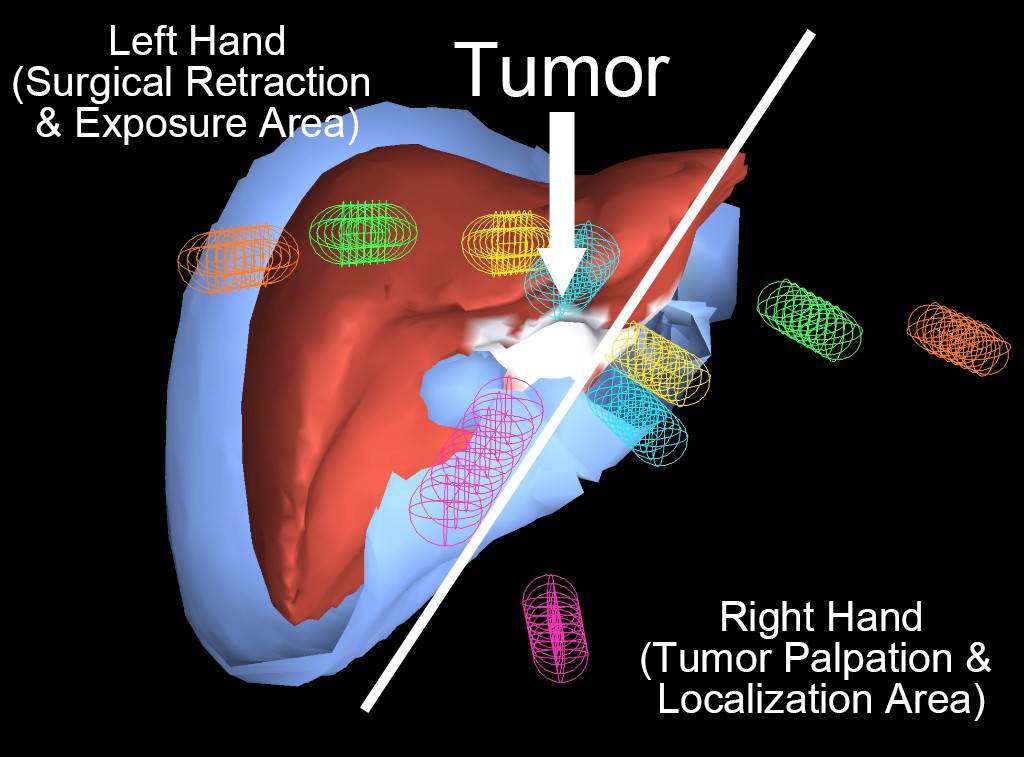
\includegraphics[width=0.96\linewidth]{system_simulation_view.png}}
\caption{Runtime screenshot of the system. The red region is the liver model, and the outer light-blue shell is the liver-shaped collision cavity used to provide spatial constraint. One side is retained as an open region to approximate the local exposure window in open surgery. The colored wireframe capsules denote fingertip proxy bodies. The left-side region corresponds to the left hand, used for pushing and retracting tissue to maintain exposure, while the right-side region corresponds to the right hand, used for lesion palpation, pressing-based comparison, and localization search.}
\label{fig:system}
\end{figure}

\begin{figure}[htbp]
\centerline{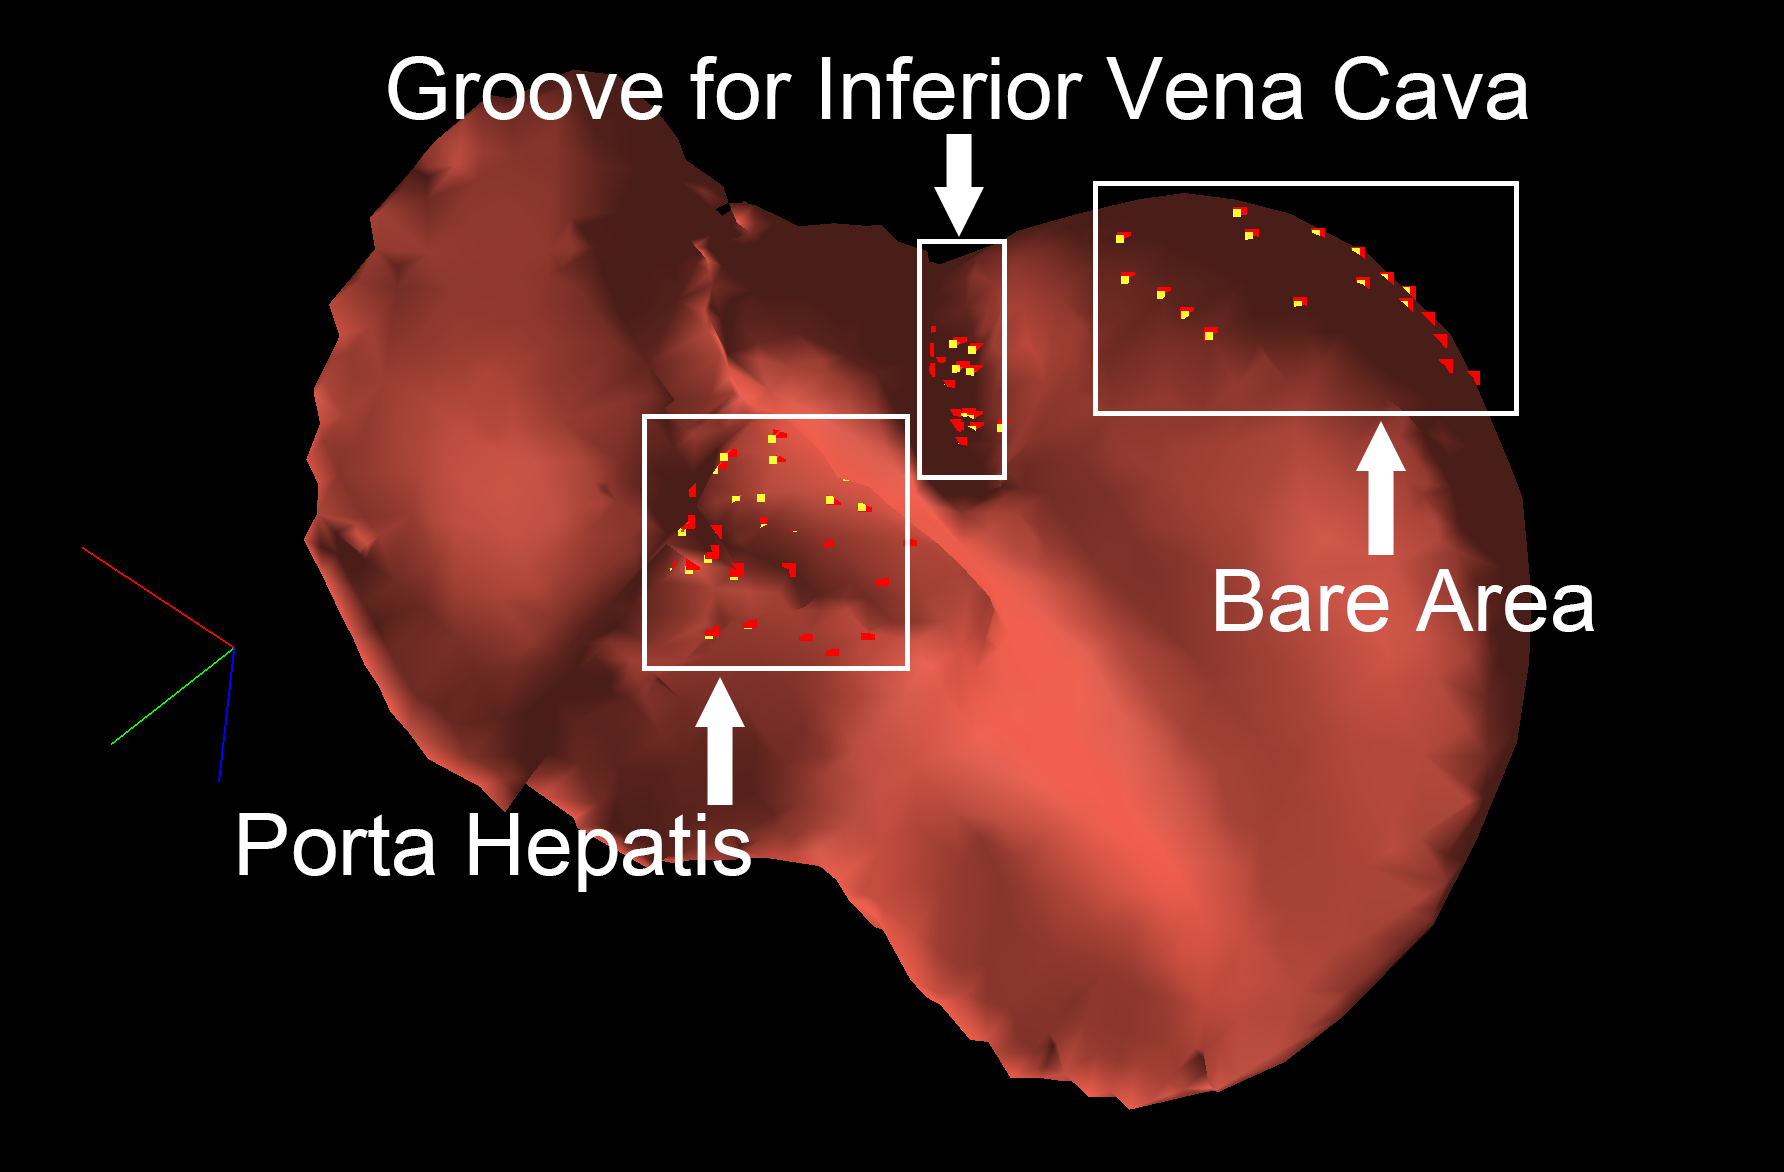
\includegraphics[width=0.82\linewidth]{liverfixedpoint.png}}
\caption{Anatomical fixation regions and fixed-node distribution in the liver model. The dotted markers denote node clusters with fixed-point constraints, corresponding to the Porta Hepatis, the Groove for the Inferior Vena Cava, and the Bare Area. These constraints approximate major anatomical attachments and suppress nonphysical rigid-body drift.}
\label{fig:fixed}
\end{figure}

\section{Experimental Design and Evaluation Metrics}
\subsection{Application-Level Technical Validation Based on a Specific Liver Model}
Although the systematic benchmark of the underlying pure algorithmic GB-cFEM framework, such as idealized tests on basic geometries, has already been published in \cite{wang2025group}, applying it to an actual medical model within a haptic loop imposes new requirements on real-time performance and physical stability because of increased model complexity. Therefore, instead of relying on the generic 3D models used in \cite{wang2025group}, this paper re-runs validation on the liver anatomical model used by the present system in order to show that the computational framework can still serve as the real-time basis of the current interactive system:
\begin{enumerate}
\item Large-deformation accuracy: displacement response of the proposed method and XPBD is compared under unified material parameters and loading conditions, using VegaFEM as the high-accuracy reference.
\item Near-incompressible volume preservation: under large dragging with different Poisson-ratio settings, the maximum and mean deviations of the volume ratio $V/V_0$ are measured.
\item Anisotropic response validation: force-displacement slopes under loading in different directions are compared to examine whether the system can stably convey direction-dependent mechanical differences.
\item Real-time performance and scalability: the physics-solver frame rate is measured at different tetrahedral scales to assess interactivity under standard CPU conditions.
\end{enumerate}

In this paper, ``XPBD Fast'' refers to a typical real-time configuration with low substeps, whereas ``XPBD Ref'' refers to a higher-accuracy reference configuration under the same mesh and the same fixation strategy but with XPBD substeps increased substantially in order to observe its error and cost near convergence.

Both XPBD configurations are reported to ensure a fair evaluation. Reporting only a low-substep setup would unfairly penalize XPBD's accuracy, while reporting only a high-substep setup would obscure its computational cost. Including both clarifies the inherent tradeoff of XPBD between real-time performance and deformation accuracy, thereby highlighting the relative advantages of the proposed method.

Unless otherwise stated, all system runtime tests, real-time demonstrations, and the formative expert evaluation in this paper were conducted on the same Mac mini (Apple, USA) with an Apple M4 Pro (12-core CPU), 24 GB memory, and macOS 26.3.1. This is emphasized because the goal of the paper is not only theoretical real-time performance, but also actual deployability on compact consumer-grade hardware. As a supplementary whole-machine observation, when the system ran continuously for 5 minutes on the same device, the wall power averaged about 52 W, compared with about 12 W at idle, indicating that the additional whole-machine power required by the real-time FEM interaction pipeline is on the order of only several tens of watts rather than a high-power workstation load.

\subsection{Formative Expert Evaluation and Observation of Lesion-Search Behavior}
One surgeon participated in the system evaluation. The participant profile is listed in Table~\ref{tab:expert}. The study protocol was approved by the ethics committee of the Institute of Science Tokyo (approval number: 2023362). The participating surgeon was informed about the study before the experiment and signed an informed-consent form.

This evaluation was a formative expert evaluation. Its goal was to identify system feasibility and engineering boundaries. The evaluation setup is shown in Fig.~\ref{fig:eval}. The expert first watched an approximately 5-minute system demonstration and then completed, in sequence, free exploration, a blind lesion-localization observation, and a usability evaluation task.

In the lesion-localization task, to reduce spatial-memory effects, different unknown lesion positions were used under the two conditions of haptics disabled and haptics enabled. The expert's search behavior and strategy changes under the two conditions were recorded for qualitative analysis of how the local stiffness cues provided by the system supported palpation judgment.

\begin{table}[htbp]
\caption{Profile of the Surgical Expert Participating in the Formative Evaluation}
\label{tab:expert}
\centering
\footnotesize
\renewcommand{\arraystretch}{1.15}
\begin{tabular}{|p{0.28\linewidth}|p{0.46\linewidth}|}
\hline
Attribute & Information \\
\hline
Professional title & Intermediate \\
\hline
Clinical experience & 7 years \\
\hline
Specialty & Surgery \\
\hline
Surgery-related experience & 2 years \\
\hline
\end{tabular}
\end{table}

\begin{figure}[htbp]
\centerline{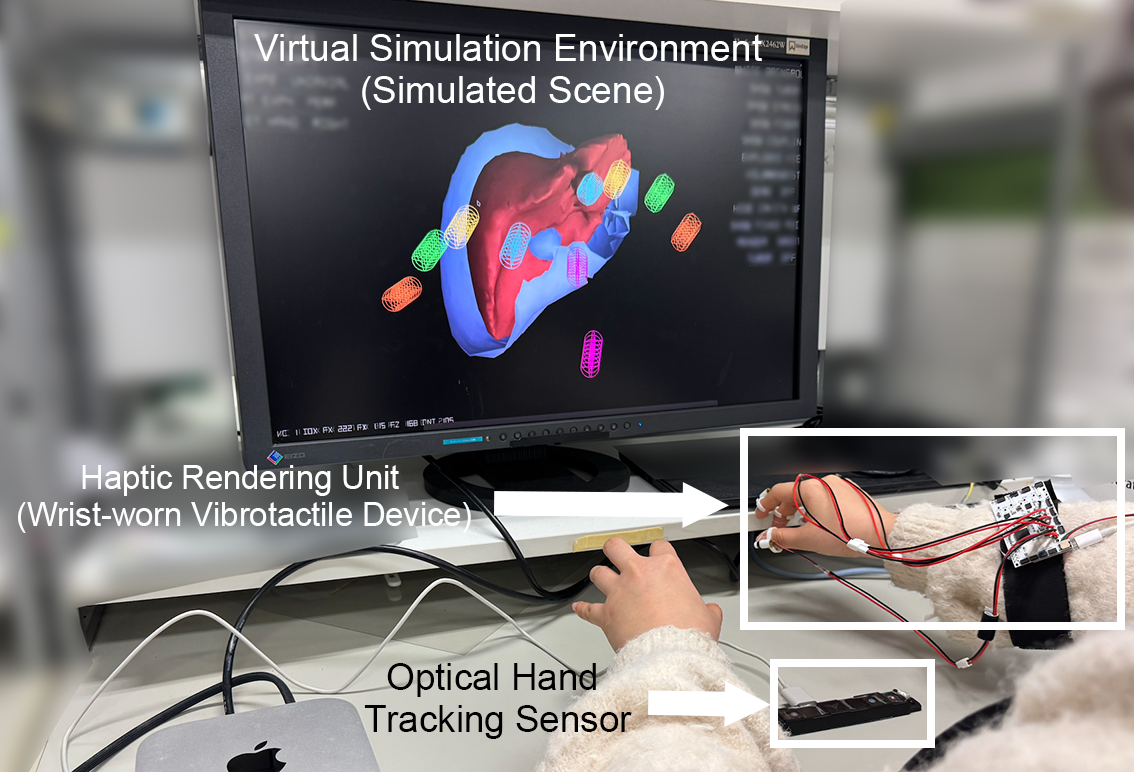
\includegraphics[width=0.88\linewidth]{expert_evaluation_setup.png}}
\caption{Formative expert evaluation setup. The participant performed virtual palpation through hand motion while receiving 1-DOF force feedback, and the screen displayed real-time liver deformation and proxy-body positions.}
\label{fig:eval}
\end{figure}

The task design and recorded contents of the formative expert evaluation are listed in Table~\ref{tab:tasks}.

\begin{table}[htbp]
\caption{Task Design and Recorded Contents of the Formative Expert Evaluation}
\label{tab:tasks}
\centering
\scriptsize
\renewcommand{\arraystretch}{1.15}
\setlength{\tabcolsep}{3pt}
\begin{tabular}{|p{0.19\linewidth}|p{0.15\linewidth}|p{0.24\linewidth}|p{0.20\linewidth}|}
\hline
Task & Goal & Condition & Recorded content \\
\hline
Task A: Free exploration & Observe interaction fidelity and naturalness & Freely touch the liver while verbalizing thoughts & Subjective evaluation and interaction behavior \\
\hline
Task B: Blind lesion localization & Observe search-behavior changes across two trials & Trial 1: haptics off; Trial 2: haptics on with a different lesion position & Operational strategy and verbal feedback \\
\hline
Task C: System usability feedback & Evaluate engineering boundaries and physical consistency & Press different regions and compare resistance differences & Semi-structured interview and Likert-scale ratings \\
\hline
\end{tabular}
\end{table}

\subsection{Metric Construction for the Formative Evaluation}
The formative evaluation in this paper records three kinds of indicators: behavioral indicators , subjective evaluation , and rating-scale scores . The assessment emphasizes qualitative observation and system-mechanism analysis in order to provide diagnostic and design guidance for the next generation of the system.

\section{Results}
\subsection{Technical Validation Results}
\subsubsection{Large-Deformation Accuracy and Real-Time Performance}
When the test was re-run on the real liver model used in this paper, with VegaFEM taken as the reference, Fig.~\ref{fig:disp} and Table~\ref{tab:disp} show that the kernel used by the present system achieved an average displacement error of about 17.9\% under three loading strengths, whereas the error of XPBD Fast exceeded 50\%. More importantly, for the liver-lesion palpation scenario considered here, which contains tens of thousands of tetrahedra, the method still achieved about 83 FPS at a computational cost of approximately 12 ms per frame, satisfying the real-time interaction requirement of the system. Although XPBD reached higher FPS at low substeps, its displacement response was overly soft, whereas the higher-accuracy configuration sacrificed real-time capability. Considering that the system test was carried out on a Mac mini M4 Pro and that the average wall power of the full machine was approximately 52 W during continuous 5-minute operation (versus about 12 W at idle), this result at least indicates that the FEM-driven pipeline is not limited to heavy computing platforms and can support actual interactive operation with only several tens of watts of additional whole-machine power.

\begin{table}[htbp]
\caption{Comparison of Large-Deformation Accuracy and Real-Time Performance}
\label{tab:disp}
\centering
\scriptsize
\renewcommand{\arraystretch}{1.15}
\setlength{\tabcolsep}{4pt}
\begin{tabular}{|p{0.20\linewidth}|p{0.13\linewidth}|p{0.13\linewidth}|p{0.13\linewidth}|p{0.12\linewidth}|}
\hline
Metric & Proposed method & XPBD Fast & XPBD Ref & VegaFEM \\
\hline
Mean displacement error & 17.9\% & 50.8\% & 43.6\% & 0\% (reference) \\
\hline
Mean runtime & 12.0 ms & 7.9 ms & 59.2 ms & -- \\
\hline
Frame rate & 83.3 FPS & 126.6 FPS & 16.9 FPS & -- \\
\hline
\end{tabular}
\end{table}

\begin{figure}[htbp]
\centerline{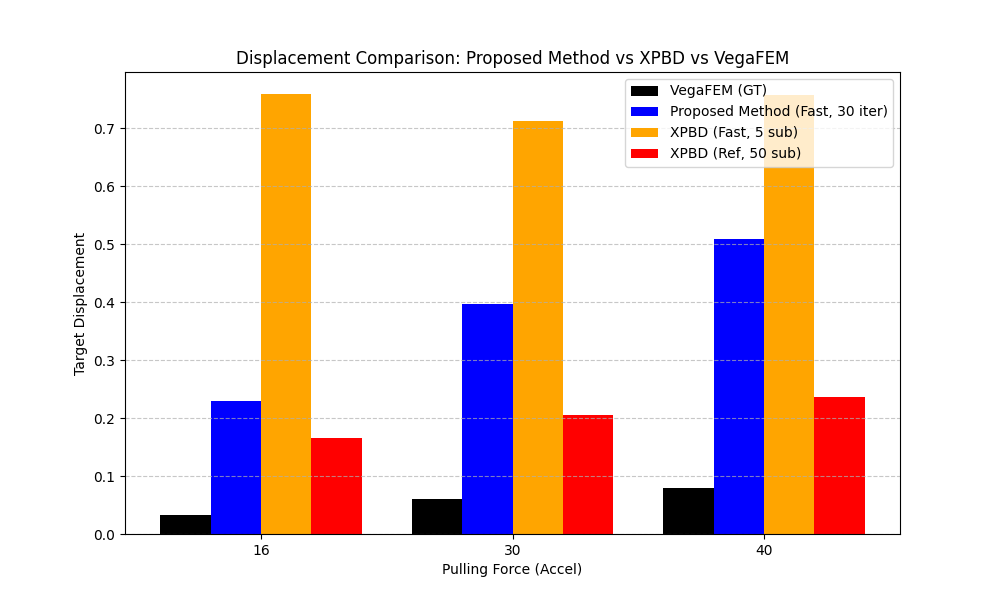
\includegraphics[width=0.96\linewidth]{displacement_comparison.png}}
\caption{Comparison of large-deformation displacement. Relative to the VegaFEM reference, the proposed method exhibits more stable displacement response than both XPBD Fast and XPBD Ref under all three loading strengths.}
\label{fig:disp}
\end{figure}

Taken together, this result provides supporting evidence for the following judgment: the simulation kernel relied upon by the present system does not simply trade accuracy for speed, but maintains a more stable stiffness representation than XPBD within an interactive operating range.

\subsubsection{Near-Incompressible Volume Preservation}
Specialized validation under the typical near-incompressible setting of a high-water-content soft tissue such as the liver shows that, as presented in Fig.~\ref{fig:volume} and Table~\ref{tab:volume}, the volume stability of the kernel used here is overall better than that of XPBD and close to the VegaFEM reference. In particular, under the $\nu = 0.47$ condition, the mean volume deviation of the tested liver model was 0.92\%, and the maximum deviation was 1.35\%, both better than XPBD.

\begin{table}[htbp]
\caption{Volume-Deviation Comparison Under Near-Incompressible Conditions}
\label{tab:volume}
\centering
\footnotesize
\renewcommand{\arraystretch}{1.15}
\begin{tabular}{|p{0.20\linewidth}|p{0.14\linewidth}|p{0.22\linewidth}|p{0.22\linewidth}|}
\hline
Method & Poisson ratio & Maximum volume deviation & Mean volume deviation \\
\hline
Proposed method & 0.28 & 1.88\% & 1.31\% \\
\hline
Proposed method & 0.47 & 1.35\% & 0.92\% \\
\hline
XPBD & 0.28 & 7.27\% & 1.84\% \\
\hline
XPBD & 0.47 & 1.59\% & 1.29\% \\
\hline
VegaFEM & 0.28 & 1.94\% & 1.28\% \\
\hline
VegaFEM & 0.47 & 1.47\% & 0.80\% \\
\hline
\end{tabular}
\end{table}

\begin{figure}[htbp]
\centerline{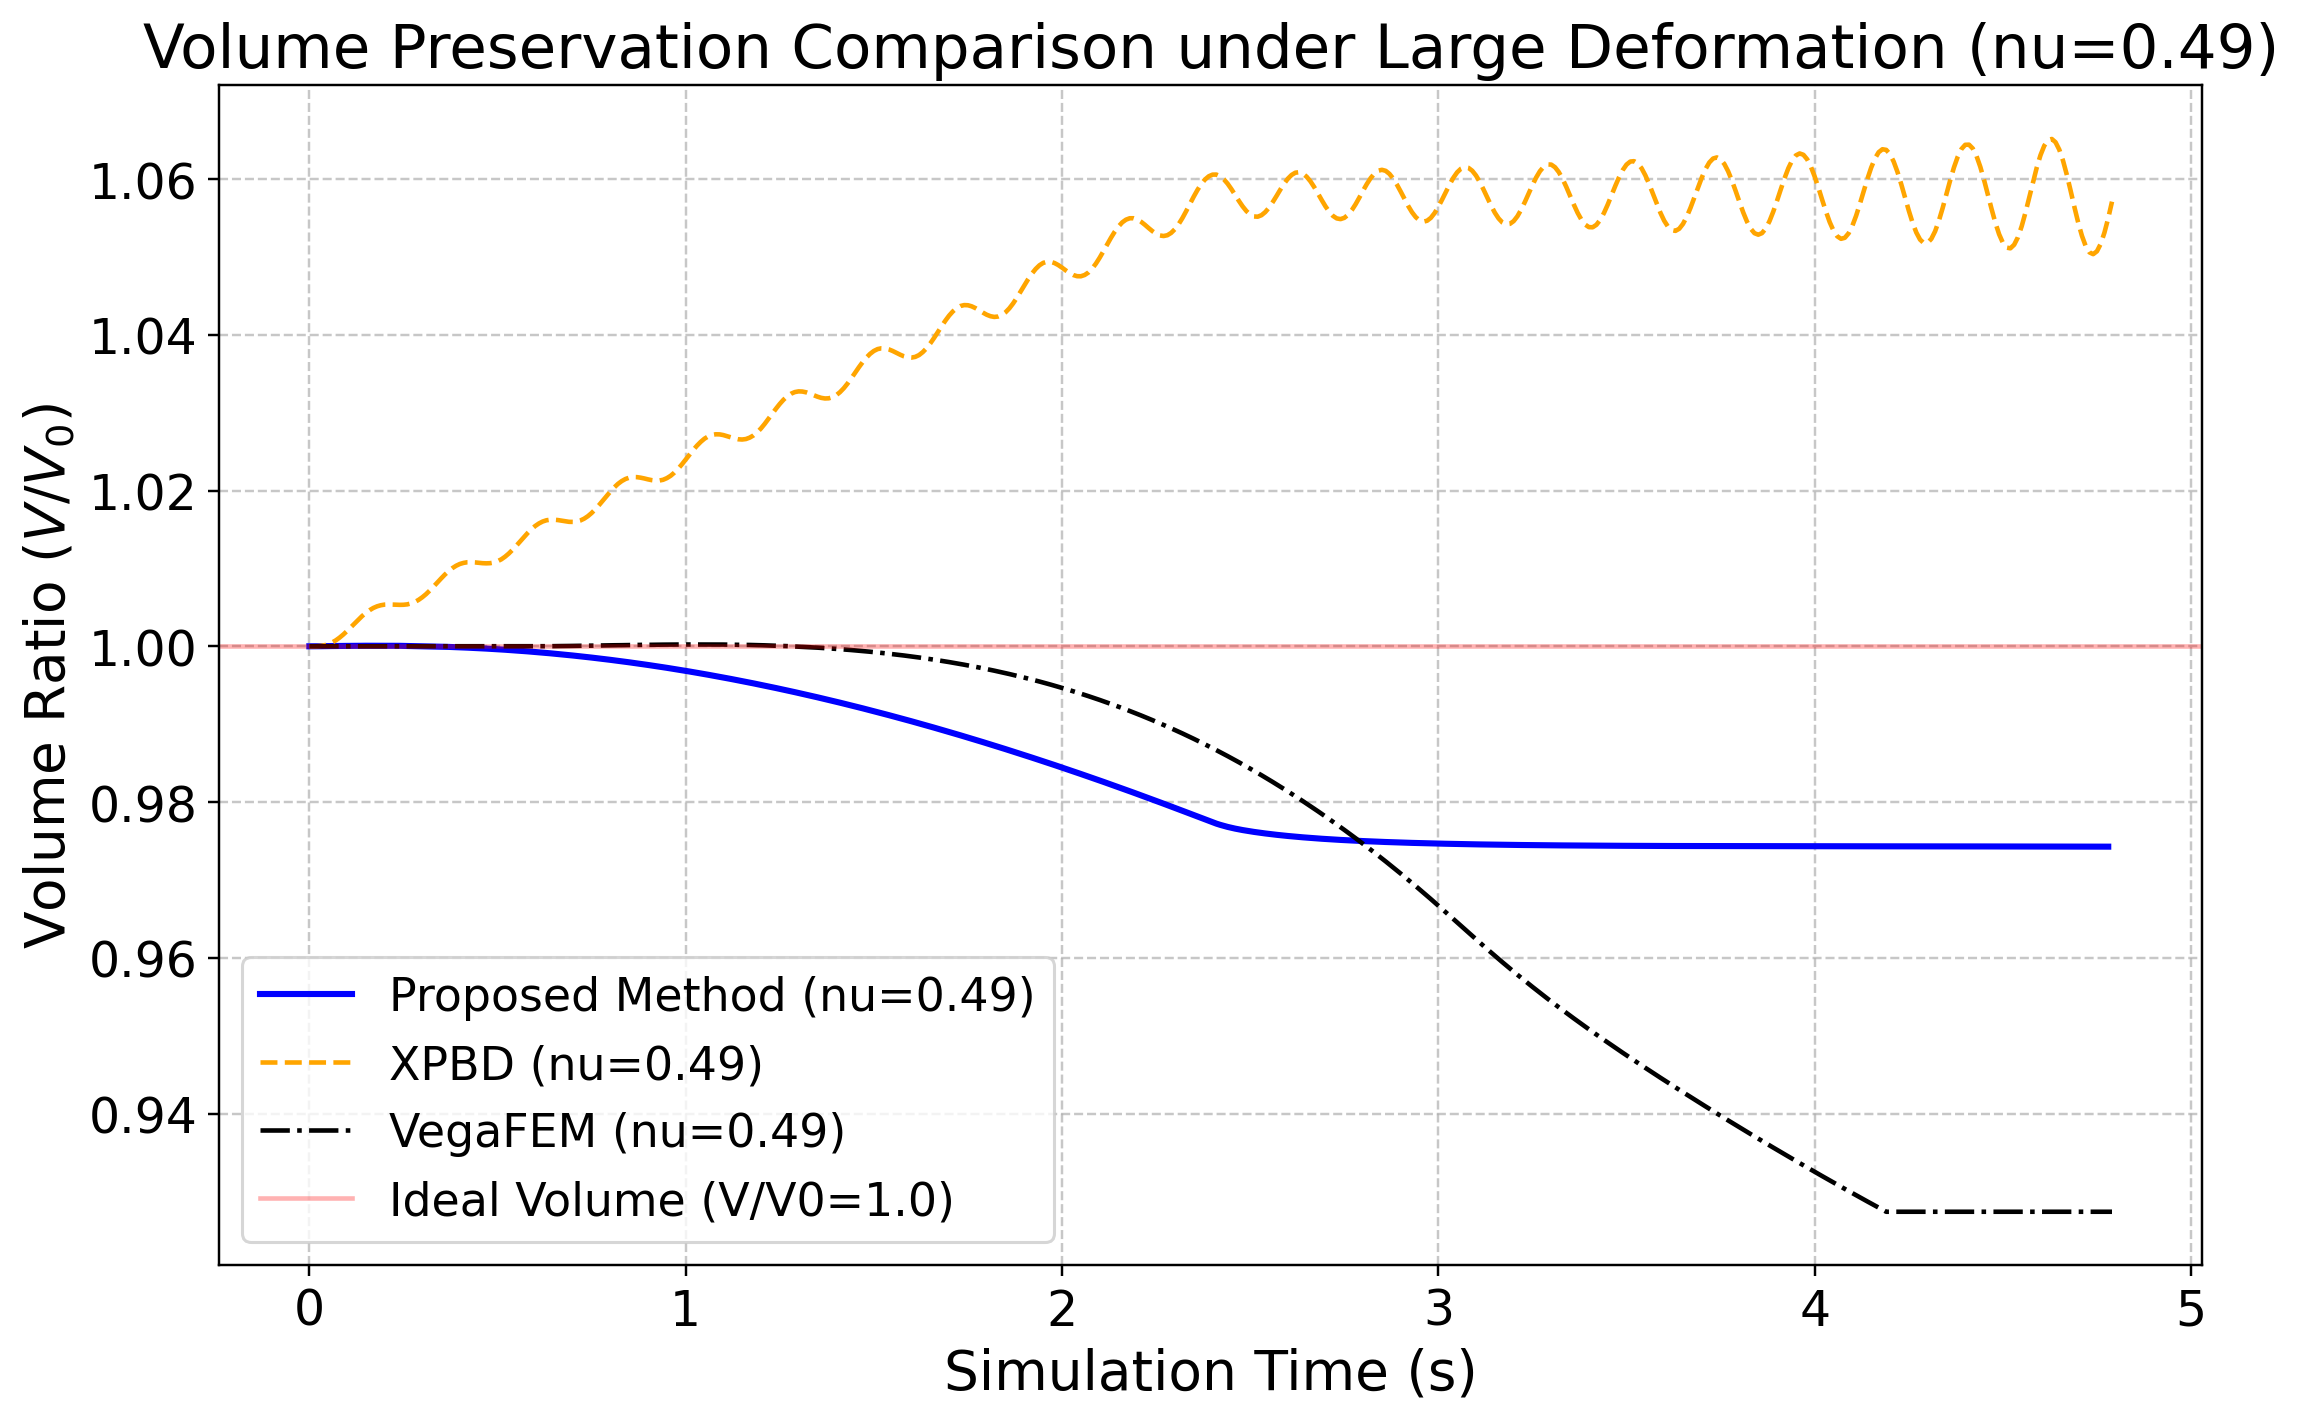
\includegraphics[width=0.96\linewidth]{volume_preservation_comparison.png}}
\caption{Comparison of volume preservation under near-incompressible conditions. The proposed method maintains small volume deviation under both Poisson-ratio settings and is overall close to the VegaFEM reference.}
\label{fig:volume}
\end{figure}

This indicates that, under the current protocol, the proposed method is less likely to produce the appearance of abnormal shrinkage or collapse under large pressing and dragging, thus providing a more consistent geometric basis for subsequent haptic mapping.

\subsubsection{Real-Time Performance and Scalability}
Following the performance framework of \cite{wang2025group}, we further evaluated the method at different mesh scales. As shown in Fig.~\ref{fig:fps} and Table~\ref{tab:fps}, the simulation kernel reached 219.24 FPS at approximately 7{,}790 tetrahedra and still maintained about 20.2 FPS at approximately 35{,}486 tetrahedra. By contrast, VegaFEM achieved only 5.52 FPS at about 18{,}245 tetrahedra, and the high-accuracy XPBD reference configuration achieved 16.27 FPS at about 20{,}061 tetrahedra.

\begin{table}[htbp]
\caption{Comparison of Real-Time Performance Across Mesh Scales}
\label{tab:fps}
\centering
\footnotesize
\renewcommand{\arraystretch}{1.15}
\begin{tabular}{|p{0.21\linewidth}|p{0.20\linewidth}|p{0.16\linewidth}|p{0.25\linewidth}|}
\hline
Method & Mesh scale & FPS & Note \\
\hline
Proposed method & 7,790 tets & 219.24 & Above real-time interaction demand \\
\hline
Proposed method & 35,486 tets & 20.2 & Maintains basic interactivity \\
\hline
XPBD Ref & 20,061 tets & 16.27 & High accuracy comes at high cost \\
\hline
VegaFEM & 18,245 tets & 5.52 & Difficult to use interactively \\
\hline
\end{tabular}
\end{table}

\begin{figure}[htbp]
\centerline{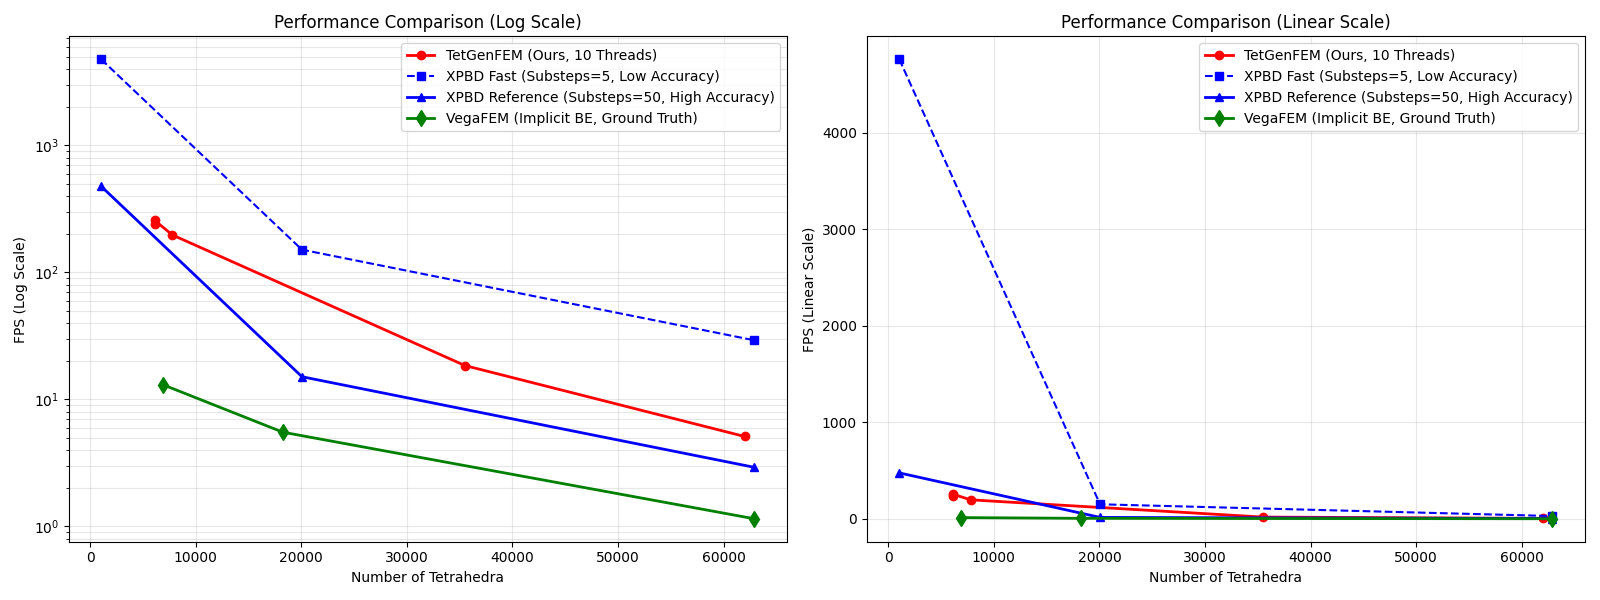
\includegraphics[width=0.96\linewidth]{comparison_fps.png}}
\caption{Overall performance trend across mesh scales. The proposed method maintains clearly better real-time performance than VegaFEM over a broad tetrahedral range and still retains basic interactivity on larger-scale models.}
\label{fig:fps}
\end{figure}

Although the mesh scales used by different methods are not matched point by point, this result is still sufficient to indicate that the GB-cFEM route used by the current system can support medical demonstration and interactive tasks on a consumer-grade CPU without relying on heavier high-end computing conditions.

\subsection{Results of the Formative Expert Evaluation and System-Usability Feedback}
\subsubsection{Interaction Fidelity During Free Exploration}
During the free-touch task, the expert participant first pressed different parts of the liver surface with multiple fingers, then attempted to lift the thin edge of the liver, and further explored the dynamic change of force feedback by varying the pressing intensity. Based on comparative palpation between the preset tumor region and normal tissue, the expert identified the engineering limitations of the system from both anatomical and physical perspectives.

The first issue concerned distortion of material behavior. The expert pointed out that the current liver soft-tissue model was overly elastic, with a feel closer to homogeneous soft gel than to fibrous biological tissue. A real liver exhibits nonlinear stiffness and is covered by a capsule, producing an initial resistance followed by constrained compression at deeper indentation. By contrast, the present model deforms too easily under compression.

The second issue concerned local perceptual differences caused by simplified anatomical constraints. The expert observed that when the liver was pushed laterally, the model exhibited global translation similar to a floating object rather than rotation constrained by anterior ligaments. In the current physical model, boundary conditions were simplified using an equivalent surface-based fixation strategy. Fixed points were assigned directly to the Porta Hepatis, the Bare Area, and the Groove for the Inferior Vena Cava to provide basal locking, superior adhesion, and posterior vertical support, respectively. Although this macroscopic fixation ensures physical stability under large deformation, the expert's feedback indicates that the lack of explicit anterior traction constraints still creates a gap between simulated feedback and clinical expectations during pushing maneuvers.

The final issue concerned deviation from the clinical interaction paradigm. The expert noted that bare-hand palpation is part of clinical diagnosis, but in surgical contexts the main interaction medium is a surgical instrument. Direct hand-tracking interaction sacrifices part of the task validity of surgical simulation and makes the experience closer to physical examination than to operative practice.


\subsubsection{Behavioral Observation in the Lesion-Localization Task}
In the initial exploration with haptic feedback disabled, the expert relied mainly on visual deformation for judgment. Observation showed that the expert first attempted light surface pressing and, after failing to obtain useful stiffness cues, gradually shifted to larger pulling motions and deeper indentation.

In the localization test with haptic feedback enabled, where the lesion was placed in a new unknown region, the expert's search behavior changed to local comparative light pressing. Verbal feedback indicated that the local differences in normal resistance provided by haptic feedback supported discrimination of the hard region. This strategy change suggests that the FEM-driven stiffness-mapping logic can provide perceptible physical cues for the lesion-search task.

The expert's operational feedback reveals the boundary between this engineering prototype and a clinical trainer. These qualitative observations play a diagnostic engineering role by providing concrete experiential guidance for future improvements in medical-simulation fidelity.

\subsubsection{Diagnosis of Engineering Constraints and Evaluation of Force-Rendering Quality}
In Task C, the expert actively performed continuous sliding exploration and deep pressing on the liver surface while cross-checking fingertip force sensation against the visual deformation shown on the screen. Based on these dynamic palpation behaviors, the expert identified a core engineering bottleneck in the system connectivity: the hardware limitation in feedback directionality. The current 1-DOF output can convey only one-directional normal resistance, while lacking tangential force and more complex reaction-force distribution. As a result, it cannot reproduce the enveloping squeeze sensation that a real finger experiences when pressed into tissue and surrounded by the material. This reflects an inherent limitation of low-dimensional hardware. The corresponding Likert-scale ratings are listed in Table~\ref{tab:likert}.

\begin{table}[htbp]
\caption{Likert-Scale Ratings of System Usability and Force-Rendering Quality}
\label{tab:likert}
\centering
\footnotesize
\renewcommand{\arraystretch}{1.15}
\begin{tabular}{|p{0.29\linewidth}|p{0.18\linewidth}|p{0.37\linewidth}|}
\hline
Evaluation dimension & Score (out of 5) & Interpretation \\
\hline
System feasibility and potential & 4/5 & The ``continuum mechanics + haptics'' system architecture was considered feasible \\
\hline
Soft-tissue mechanical expression & 4/5 & The stiffness settings of the physical engine could be effectively mapped into haptic cues \\
\hline
Force-feedback realism & 3/5 & The physical limitation of single-DOF hardware dimensionality and refresh behavior was revealed \\
\hline
\end{tabular}
\end{table}

According to the Likert-scale scores in Table~\ref{tab:likert}, the system received positive ratings in ``architectural feasibility'' and ``soft-tissue mechanical expression'' (4/5), while the score for ``force-feedback realism'' was only moderate (3/5). This result confirms the successful integration of the system's data flow while identifying future engineering challenges in hardware frequency response and feedback dimensionality.

\section{Discussion}
\subsection{From Algorithm Validation to System-Prototype Evaluation}
While the prior GB-cFEM work addressed real-time large-deformation physical solving and the previous haptic-device work addressed lightweight fingertip output, the contribution of this paper lies in the task-oriented integration of a medical palpation scenario, the normal-force-mapping closed loop, deployment on consumer-grade hardware, and formative expert diagnosis.

This paper focuses on validating the feasibility of a palpation interaction system driven by a physical kernel. The application-level technical validation provides supporting evidence that the simulation kernel can support real-time stiffness expression on a medical model, while the formative evaluation identifies the boundaries of the model as an interactive prototype through walkthrough-based diagnosis. The issues highlighted in the evaluation, including simplified anatomical constraints, the absence of material nonlinearity, and the directional limitation of 1-DOF output, are not merely generic engineering limitations. They directly affect the judgment logic of the core task of lesion localization.

First, the absence of material nonlinearity makes the model deform too easily under deep compression, weakening the operator's ability to probe deep lesions based on progressive resistance. Second, simplified anatomical constraints allow global translation during lateral pushing, where organ displacement masks local hardness abnormalities and interferes with the recognition of marginal lesions. Third, the 1-DOF normal-force limitation lacks tangential cues, preventing the perception of resistance gradients during sliding and forcing the operator to rely on dense vertical pressing to outline lesion boundaries. Overall, these findings reveal how engineering simplifications alter palpation behavior—nuances difficult to capture through numerical tests alone—and provide concrete targets for future system evolution.

\subsection{Application Focus and Future Evolution of the System}
For the test scenario of liver lesion localization, the current system expresses lesion characteristics through normal-force-based stiffness feedback. At the same time, what is validated here is not an isolated implementation for one specific liver model, but a transferable way of organizing the system. As long as the target task also depends on differences in stiffness across tissue regions, contact-reaction cues, and real-time updatable soft-tissue deformation, the architecture of ``GB-cFEM physical kernel + material stiffness that varies by region + haptic mapping'' may be extended to other soft-tissue palpation or lesion-search scenarios. Of course, such extension is not unconditional and still requires organ-specific remodeling of geometry, boundary constraints, material parameters, and interaction paradigm. To improve overall simulation immersion, future development should incorporate nonlinear material models with capsule effects and more realistic anatomical constraints for stronger organ anchoring. Additionally, the system can be extended to support instrument-based workflows and enhance the 1-DOF haptic feedback with better tangential compensation and control continuity.

\subsection{Future Research Directions}
Future work should examine task validity and training effectiveness with a larger sample, but the current scope remains focused on system-prototype design and technical feasibility. The next engineering iteration will prioritize refining ligament and abdominal boundaries for better macroscopic support, integrating surgical-instrument proxies to correct the interaction paradigm, and optimizing synchronization between the physics engine and the haptic loop to ensure smoother force rendering.

\section{Conclusion}
This paper proposes and implements a task-oriented haptic training prototype to verify the system connectivity and engineering feasibility of integrating a GB-cFEM physical engine with a haptic interface. By combining GB-cFEM-based real-time soft-tissue simulation with haptic mapping and using liver lesion localization as a concrete test scenario, the study realizes the transformation of a physical simulation kernel into an interactive feedback engine.

The technical validation provides application-level evidence regarding robustness, real-time performance, and computational economy on a medical model, showing that the system can run stably on ordinary consumer-grade hardware. However, these comparative results should still be understood as comparative validation for a system prototype rather than as a fully standardized cross-method benchmark. The evaluation in this paper is a formative expert evaluation whose goal is to identify system feasibility and engineering boundaries rather than to prove training effectiveness. The assessment by a single surgical expert identifies the engineering challenges and boundaries that must be addressed before the prototype can move toward a high-fidelity clinical trainer, including richer nonlinear material properties, more complete anatomical constraints, and expanded feedback dimensionality.

\DIFdelbegin \DIFdel{Overall, this paper validates the feasibility of a ``continuum physics computation + task-oriented haptic feedback '' architecture. Through system-level diagnosis in a formative evaluation, the study clarifies the current design limitations and engineering boundaries of the system and provides engineering evidence and design insight for exploring lightweight palpation solutions and building the next generation of medical physical-interaction systems}\DIFdelend \DIFaddbegin \DIFadd{In summary, the real-time haptic simulation prototype proposed and validated in this study matches the actual demands of modern medical education. By integrating interactive finite element physics computation with a haptic feedback interface, this system responds to the hardware accessibility need for deploying high-frequency simulation training in routine teaching environments, and it meets the educational standards of improving the learning efficiency of practical medical skills through high-information physical feedback}\DIFaddend .

\section*{Acknowledgment}
ChatGPT (OpenAI) and Gemini (Google) were used for editorial support.

\bibliographystyle{IEEEtran}
\bibliography{../Frontiers_LaTeX_Templates/bibtex/references}

\EOD

\end{document}
